\documentclass[sigplan,nonacm,natbib=false]{acmart}

% Preprint version — remove ACM copyright/conference boilerplate
\settopmatter{printacmref=false}
\renewcommand\footnotetextcopyrightpermission[1]{}
\pagestyle{plain}

\usepackage{booktabs}
\usepackage{listings}
\lstset{breaklines=true, basicstyle=\small\ttfamily, language=Python}

\setlength{\emergencystretch}{3em}
\sloppy

\begin{document}

\title{EvolveTool-Bench: Evaluating the Quality of LLM-Generated Tool Libraries as Software Artifacts}

\author{Alibek T. Kaliyev}
\affiliation{%
  \institution{The University of Texas at Austin}
  \city{Austin}
  \state{TX}
  \country{USA}
}
\email{alibek.kaliyev@utexas.edu}

\author{Artem Maryanskyy}
\affiliation{%
  \institution{Independent Researcher}
  \city{San Francisco}
  \state{CA}
  \country{USA}
}
\email{artem.maryanskyy@users.noreply.github.com}

\begin{abstract}
LLM agents increasingly synthesise their own tools at runtime --- Python functions, API clients, data parsers --- and accumulate them in persistent libraries. The field evaluates these systems almost exclusively by downstream task completion, which is analogous to judging a software engineer by whether their code compiles: it captures whether the program runs, not whether it is correct, reusable, or safe to keep. We introduce \textsc{EvolveTool-Bench}, a diagnostic framework that treats LLM-generated tool libraries as software artifacts and evaluates them at the library level using independent hidden tests, adversarial inputs, and explicit regression tasks. The framework defines a per-tool Tool Quality Score over correctness, robustness, generality, and code quality, six library-level metrics (reuse, redundancy, quality gate, utilization, composability, regression stability), and a composite EvolveTool Score combining them with a refinement-cost penalty. We evaluate six contemporary tool-creation protocols --- no-evolution, one-shot creation, strategy-only adaptation, CREATOR-style author-execute-rectify, ToolMaker-style scaffolded synthesis, and full code-level evolution with sandbox validation --- across three code-execution domains (proprietary data formats, API orchestration, numerical computation), 99 tasks per configuration, and two Claude models, with multi-seed coverage on the main Sonnet configurations. Three findings stand out. First, task completion alone fails to distinguish systems: across protocols TC clusters in a 63--72\% band on Sonnet, while library health spans a much wider range. Second, when held to independent hidden tests rather than self-generated ones, no protocol produces tools that reliably pass: per-tool correctness across every system we evaluate is in the 0--3\% range, even when the system reports task completion above 60\%. We argue this is the central diagnostic finding of the benchmark --- current LLM tool synthesis is far less robust than task-completion numbers imply. Third, a ``reuse paradox'' surfaces under multi-seed analysis: the system with the highest raw reuse (72.2\%) reuses defective tools 38.9\% of the time; reuse decomposition is essential. We also document that library health and task completion are statistically orthogonal at session granularity ($\rho = -0.03$ over 144 sessions), validating multi-dimensional reporting over a single composite. We release \textsc{EvolveTool-Bench} as an open framework with preserved per-tool artifacts, an artifact gallery, and a skill-bundle evaluation track for systems that emit Anthropic-Claude-Skills-style multi-file artifacts. The contribution is a diagnostic methodology for the next phase of self-evolving agents, not a leaderboard.
\end{abstract}

\maketitle

\section{Introduction}

LLM agents increasingly generate executable software artifacts at runtime (Python functions, API clients, data parsers) and accumulate them in persistent libraries variously called \emph{tools}, \emph{skills}, or \emph{actions}. This capability appears across diverse systems: VOYAGER~\cite{wang2023voyager} synthesizes code skills in Minecraft, CREATOR~\cite{qian2023creator} uses tool creation as a reasoning strategy, LLMs as Tool Makers~\cite{cai2023latm} separates tool-making from tool-using, EvoSkill~\cite{alzubi2026evoskill} evolves structured skill folders via failure analysis, and ARISE~\cite{kaliyev2026arise} provides framework-agnostic middleware for tool synthesis with sandboxed validation. As reusable procedural knowledge is increasingly packaged, shared, and composed across agents, the quality of these generated artifacts becomes a first-order concern.

From a software engineering perspective, each of these systems is an \emph{automated code generator} whose output accumulates into a growing codebase. Yet they are evaluated exclusively on task success, analogous to judging a software engineer solely by whether their code runs, ignoring maintainability, duplication, test coverage, regression, and technical debt. In practice, skill libraries can pass downstream benchmarks while accumulating redundant functions, failing on edge cases, breaking previously working capabilities, and never reusing existing code. Recent work confirms the risk: SkillsBench~\cite{skillsbench2026} found that self-generated skills \emph{hurt} agent performance by 16.2 points in roughly one-third of tasks. \textbf{No existing benchmark measures \emph{why} this happens}: whether the degradation stems from incorrect implementations, redundant code, regression, or failed reuse.

We present \textsc{EvolveTool-Bench}, a diagnostic framework that treats LLM-generated tool and skill libraries as software artifacts and evaluates them at the library level. The framework is system-agnostic: any tool-creating or skill-creating agent can be evaluated against the same tasks and metrics. Our contributions:

\begin{enumerate}
\item \textbf{A library-level metric framework.} We define a per-tool Tool Quality Score (TQS) over correctness, robustness, generality, and code quality, plus six library-level metrics --- reuse rate, redundancy, quality gate, utilization, composability, and regression stability --- and a composite EvolveTool Score (ETS) that combines them with a refinement-cost penalty.

\item \textbf{An evaluation harness with independent validation.} Hidden unit tests, adversarial inputs, and held-out generality probes run in sandboxed subprocesses, providing quality assessment that does not depend on the system's own self-validation. Explicit regression tasks measure whether library growth breaks previously working behaviour.

\item \textbf{Structured diagnostic sessions.} Sequences of 11 tasks with known dependency relationships (seed, gap, variant, compose, regress, adversarial; Figure~\ref{fig:overview}) make it possible to measure reuse recognition, function composition, and library stability as the codebase grows.

\item \textbf{A multi-protocol evaluation revealing failure modes hidden by task completion.} We evaluate six tool-creation protocols across three code-execution domains and surface findings invisible to TC-only evaluation: per-tool correctness in the 0--3\% range across all systems under independent testing despite TC$>$60\%, a reuse paradox where high reuse rates mask defective-tool reuse, and an empirical orthogonality between library health and task completion ($\rho{=}-0.03$ over 144 sessions).
\end{enumerate}

\section{Related Work}

\paragraph{Quality of LLM-Generated Code.} Tool-Genesis~\cite{xia2026toolgenesis} evaluates one-shot tool creation with surface compliance, schema-F1, and unit test pass rates, all per-artifact metrics with no library-level evaluation. SkillsBench~\cite{skillsbench2026} is the closest work in motivation: it evaluates whether curated skills improve agent task success and finds that self-generated skills \emph{degrade} performance by 16.2 points in $\sim$33\% of tasks, a result that directly motivates our work. However, SkillsBench uses static, pre-curated skill sets and measures only the downstream effect (did performance improve?), not the \emph{cause} (is the skill buggy? redundant? regression-inducing?). Our benchmark complements SkillsBench by providing the diagnostic layer: per-tool quality scores, library-level metrics, and structured sessions that isolate \emph{why} a skill library helps or hurts. Our ``reuse paradox'' (38.9\% incorrect reuse in Code-Evol/Sonnet over 4 seeds; \S\ref{sec:reuse_analysis}) offers one explanation for SkillsBench's finding: agents reuse skills they correctly identify as relevant but that contain implementation defects. NofunEval~\cite{singhal2024nofuneval} evaluates non-functional aspects of LLM-generated code (efficiency, maintainability) on isolated samples; our work differs by evaluating non-functional properties at the library level, across a growing codebase with reuse and regression. CRAFT~\cite{yuan2023craft} retrieves from specialized toolsets but does not measure the quality of the toolset itself. Berlot-Attwell et al.~\cite{berlotattwell2026} evaluate library learning quality in program synthesis, measuring whether learned abstractions generalize. Their work is similar in spirit to ours, though focused on program synthesis rather than agent skill evolution. None of these works measure redundancy, regression, or reuse across a growing codebase.

\paragraph{Self-Evolving Agent Frameworks.} VOYAGER~\cite{wang2023voyager} demonstrates lifelong skill acquisition in Minecraft, evaluated by exploration metrics. EvoSkill~\cite{alzubi2026evoskill} evolves textual skill folders through failure-driven feedback, evaluated by downstream accuracy. ARISE~\cite{kaliyev2026arise} synthesizes executable Python functions with auto-generated test suites, validates them in isolated sandboxes, and supports iterative refinement. Each generates software artifacts that accumulate into a skill library, but none evaluate the quality of the resulting library, a gap our benchmark fills.

\paragraph{Software Engineering Benchmarks for Agents.} ToolBench~\cite{qin2023toolbench}, AgentBench~\cite{liu2024agentbench}, and ToolComp~\cite{toolcomp2025} evaluate agents using pre-defined tool sets. Vending-Bench~\cite{backlund2025vendingbench} tests long-horizon coherence with fixed tools. None evaluate agents that \emph{generate} their own tools, and none apply software quality metrics to the generated artifacts.

\paragraph{Program-Synthesis Library Learning.} A separate lineage of work, originating in program synthesis rather than LLM agents, has long measured the quality of \emph{learned libraries}. DreamCoder~\cite{ellis2021dreamcoder} bootstraps inductive program synthesis by alternately compressing solved problems into a library and solving harder ones from it, evaluating the library by compression ratio and downstream solve rate. Stitch~\cite{bowers2023stitch} provides a faster top-down algorithm for the same abstraction-discovery problem; babble~\cite{cao2023babble} uses e-graphs and anti-unification for the same goal. AbstractBeam~\cite{zenkner2024abstractbeam} brings library learning to bottom-up bottom-up synthesis. Leroy~\cite{bellur2024leroy} extends library learning to imperative languages. Berlot-Attwell et al.~\cite{berlotattwell2026} recently argued that much purported library learning in LLM-based program synthesis fails when one accounts properly for compute and behaviour. Our benchmark differs in two ways: (i) the artifacts under test are \emph{LLM-generated tools for natural-language-described tasks}, not abstractions extracted from solved programs, and (ii) we measure correctness against \emph{hidden tests} alongside compression-style reuse, so a library that achieves high reuse with defective tools (our ``reuse paradox'') is not awarded the same score as one with correct reuse. We see EvolveTool-Bench as complementary to this lineage rather than competing with it.

\paragraph{Concurrent Tool/Skill Benchmarks.} Two contemporaneous benchmarks deserve direct comparison. The ToolMaker pipeline of W{\"o}lflein et al.~\cite{wolflein2025toolmaker} introduces TM-Bench, which evaluates whether an agent can convert a research paper into a runnable tool that an LLM-as-judge can verify. CoEvoSkills~\cite{zhang2026coevoskills} pairs skill generation with adversarial verification and reports skill-level pass rates. Both focus on per-tool correctness; neither evaluates redundancy, regression, utilization, or composability of the resulting \emph{library}. Tool-Genesis~\cite{xia2026toolgenesis} is the closest in spirit (it evaluates schema-F1 and unit-test pass rates of generated tools), but again at the per-tool level. EvolveTool-Bench's contribution is orthogonal: we evaluate the library as a software artifact, and any of these systems could be plugged into our harness as an additional configuration.

\paragraph{Gap.} No existing benchmark measures redundancy, reuse, regression, composition, or code quality of self-evolved skill libraries as software artifacts \emph{at the library level}. SkillsBench shows that skills can hurt; we provide the diagnostic framework to explain \emph{why}. \textsc{EvolveTool-Bench} fills this gap with a system-agnostic evaluation framework.

\section{Benchmark Design}

We first define key terms used throughout. A \emph{session} is a fixed sequence of 11 tasks executed in order with shared library state. A \emph{task} is a single problem instance presented to the agent, consisting of a natural-language description, expected output format, and verification criteria. A \emph{dependency} is a directed relationship where a later task is designed to be solvable using artifacts created during an earlier task. All tasks require actual Python code execution; no task can be solved by text-only reasoning.

The benchmark evaluates two kinds of synthesized artifact, which differ in granularity:

\begin{itemize}
\item A \textbf{tool} is a single Python function with documentation. This is the unit most existing systems (VOYAGER, CREATOR, ToolMaker, ARISE) emit, and the unit that most of \S\ref{sec:results} reports on. The library $\mathcal{L}$ is the set of such tools available to the agent in a given session.

\item A \textbf{skill} is a richer multi-file bundle: a callable function paired with a \texttt{SKILL.md} description, auto-generated unit tests, and a \texttt{metadata.json} manifest with name, version, dependencies. This is the format used by Anthropic Claude Skills and by CoEvoSkills~\cite{zhang2026coevoskills}. We extend the evaluator to score skill bundles on structure compliance, documentation quality, and metadata correctness alongside the four TQS dimensions (\S\ref{sec:skill_eval}).
\end{itemize}

Most baselines we evaluate synthesize tools; in \S\ref{sec:skill_eval} we add a dedicated skill-format track in which the expected artifact is a skill bundle rather than a single function. We use \emph{artifact} as the umbrella term for either.

\begin{figure*}[t]
\centering
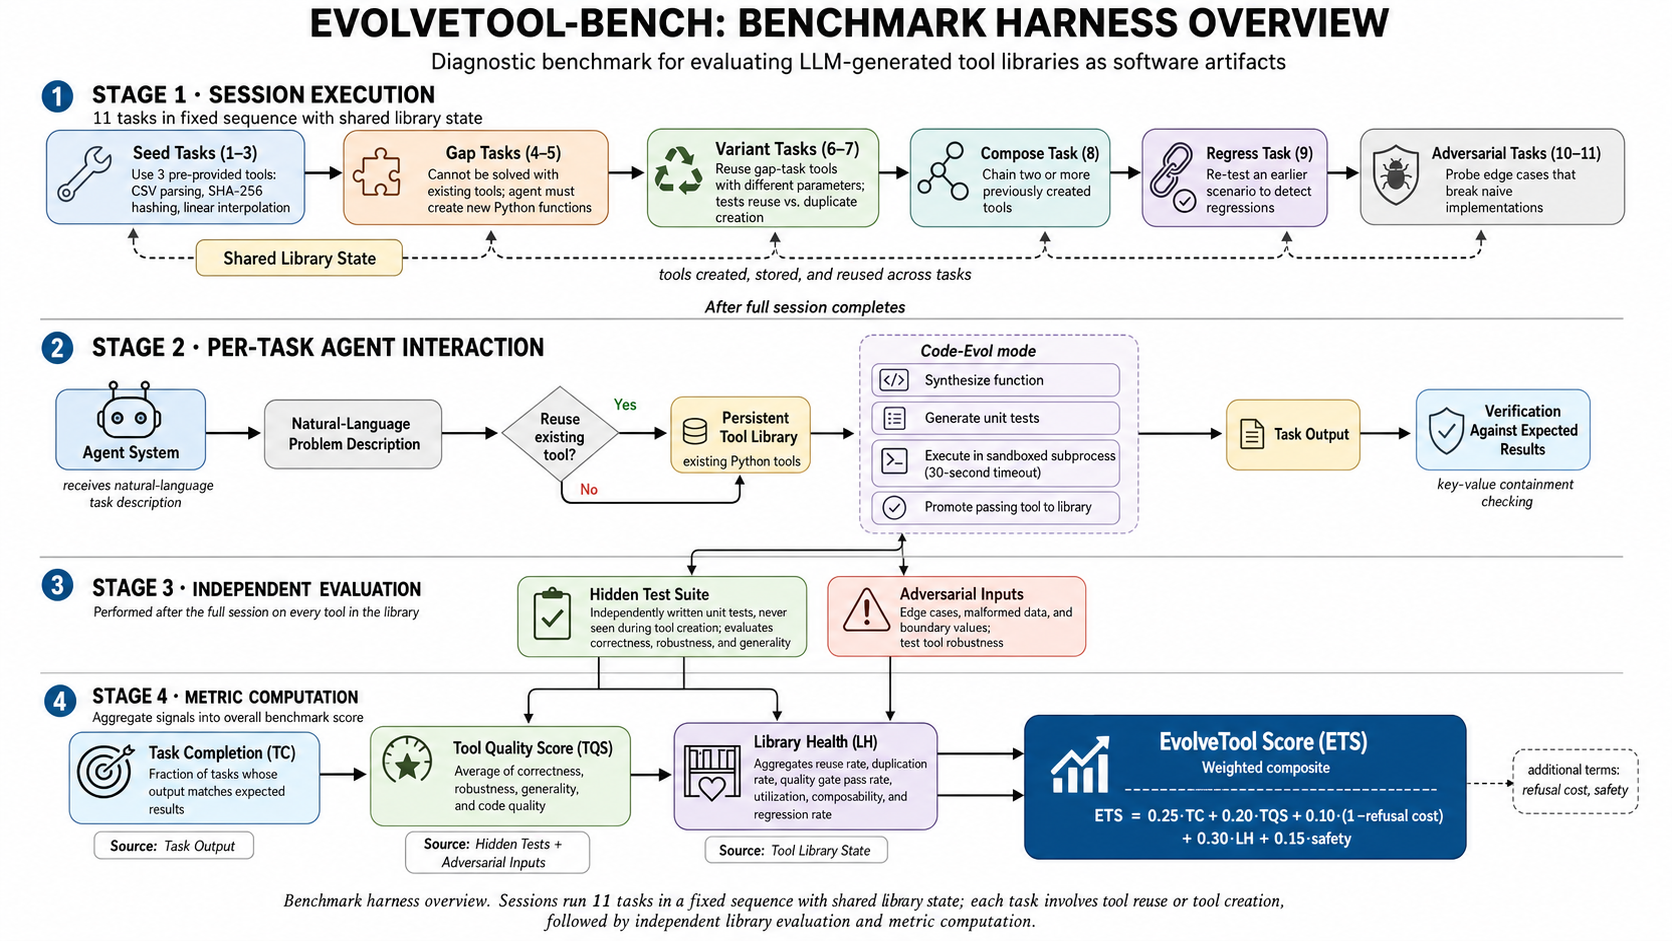
\includegraphics[width=\textwidth]{fig_overview.png}
\caption{Benchmark harness overview. \textbf{Top:} each session runs 11 tasks in a fixed sequence; annotations show what each task type tests. \textbf{Middle:} the agent system receives each task as natural language, creates or reuses Python tools in a persistent library, and produces output. After the session, hidden tests and adversarial inputs independently evaluate the library. \textbf{Bottom:} four metrics are computed: task completion (TC) from outputs, per-tool quality (TQS) from hidden tests, library health (LH) from library state, and the composite EvolveTool Score (ETS).}
\label{fig:overview}
\end{figure*}

Figure~\ref{fig:overview} shows the benchmark harness. Each session runs 11 tasks in a fixed order; the agent system receives each task as a natural-language description, uses or creates Python tools in a shared library, and produces output verified against expected results.

\subsection{Task Session Structure}

Each session contains 11 tasks in six categories with known dependency relationships (Table~\ref{tab:task_types}). This structure mirrors software engineering workflows: seed tasks test existing code, gap tasks require new implementation, variant tasks test code reuse, compose tasks test function composition, regress tasks detect regressions, and adversarial tasks probe edge cases.

\begin{table}[t]
\centering
\footnotesize
\begin{tabular}{llp{3.2cm}}
\toprule
\textbf{Type} & \textbf{N} & \textbf{SE Analog} \\
\midrule
Seed & 3 & Use existing library \\
Gap & 2 & Implement new feature \\
Variant & 2 & Reuse vs.\ rewrite \\
Compose & 1 & Function composition \\
Regress & 1 & Regression testing \\
Adversarial & 2 & Edge case / fuzz testing \\
\bottomrule
\end{tabular}
\caption{Task types and their software engineering analogs. Each session follows a fixed sequence enabling controlled measurement of library evolution.}
\label{tab:task_types}
\end{table}

The task ordering within each session is deliberate. Seed tasks (1--3) establish baseline functionality using pre-provided tools. Gap tasks (4--5) present problems that \emph{cannot} be solved with existing tools, forcing the system to create new ones. Variant tasks (6--7) present problems solvable by the tools created in gap tasks with different parameters, the key test of whether the system recognizes a reuse opportunity or wastefully creates a duplicate. The compose task (8) requires chaining two or more previously created tools. The regress task (9) re-tests an earlier scenario to detect regressions introduced by library growth. Adversarial tasks (10--11) probe edge cases designed to break naive implementations.

\paragraph{What the regress task measures (and what it does not).}
Real software regularly changes interfaces in response to evolving requirements; ``different behaviour'' is not always ``regression.'' We restrict $\delta$ to \emph{behaviour-preserving} regressions: each regress task replays the \emph{exact same input/output contract} as an earlier task in the session, with no new requirements injected. The expected output is unchanged, so if the agent's answer is now wrong, the only explanation is that library growth (a new tool, a refinement, or a wrapper) has broken a previously-working capability. This deliberately excludes the legitimate-interface-change case. A complementary ``requirement-evolution'' axis, in which a later task changes the contract on purpose and asks whether the agent migrates cleanly, is an extension we leave to future work; the current $\delta$ should be read narrowly as \emph{regression under fixed requirements}.

\subsection{Reuse Detection}
\label{sec:reuse}

The reuse metric measures whether the agent recognizes that an existing tool can solve a new task. Before each task, the harness records the current library ($\mathcal{L}_{\text{before}}$). After the task, it identifies newly created tools ($\mathcal{L}_{\text{new}}$) and checks whether any tool \emph{used} by the agent was from the pre-existing set. Formally, for variant and regress tasks:

\begin{equation}
\text{reused}(t) = \exists\, f \in \text{tools\_used}(t) : f \in \mathcal{L}_{\text{before}} \setminus \mathcal{L}_{\text{new}}
\end{equation}

This measures the \emph{behavioral signal}: did the system attempt reuse? This is measured independently of whether the trajectory was correct. We further decompose reuse into \emph{correct reuse} (reused tool AND task passed) and \emph{incorrect reuse} (reused tool AND task failed); see Section~\ref{sec:reuse_analysis}.

\subsection{Composition Tasks}
\label{sec:compose}

Each compose task has an explicit \texttt{composes\_tasks} field referencing prior task IDs whose tools must be chained. For example, an API orchestration compose task references \texttt{["gap\_1", "gap\_2"]}: the agent must chain the authentication tool (from gap\_1) with the pagination tool (from gap\_2) to fetch and aggregate all users.

We do \emph{not} guarantee that the prerequisite tools exist in the library. If the system failed to create them during earlier gap tasks, the compose task becomes harder; it must solve everything from scratch. This is realistic: a fragile library makes composition harder, and the metric captures this cascading effect.

\subsection{Domains}
\label{sec:domains}

We design three domains with tasks that require \emph{actual code execution} and cannot be solved by pattern-matching against training data.

\paragraph{Domain A: Data Transformation (5 sessions, 55 tasks).} Five proprietary binary formats designed to have no overlap with LLM training data: custom binary serialization with CRC checksums (ABR), run-length encoded matrices (RLE), a schema validation language (VDL), binary log format with variable-length entries (QLOG), and nested serialization with parity-based error correction (TPACK).

\paragraph{Domain B: API Orchestration (1 session, 11 tasks).} A mock HTTP server implementing HMAC-timestamp authentication and XOR-encrypted cursor pagination. Tasks require the agent to authenticate, paginate through results, handle cursor decryption, and compose these capabilities.

\paragraph{Domain C: Numerical Computation (3 sessions, 33 tasks).} Custom scientific computing formats for nonlinear curve fitting (ARCFIT), signal processing with FFT-based spectral analysis (ARCSIG), and constrained optimization with boundary analysis (ARCOPT).

\subsection{Running Example: API Orchestration}

We walk through a single API orchestration session to illustrate how the benchmark works in practice.

\paragraph{Seed task 1.} The agent receives: ``Check if the API server is healthy by making a GET request to \texttt{http://127.0.0.1:18080/health}.'' The pre-loaded \texttt{http\_get} tool handles this. All systems pass.

\paragraph{Gap task 4.} The agent receives: ``Authenticate with the API. First, GET \texttt{/auth-info} to obtain the secret and algorithm. Then compute an HMAC-SHA256 signature over \texttt{timestamp:path} and include it as a header.'' No existing tool computes HMAC signatures. Code-Evol detects the failure, synthesizes \texttt{compute\_hmac(secret, message) -> str}, generates 5 tests (valid inputs, empty string, unicode), runs them in a sandbox (all pass), and promotes the tool to the library. No-Evolution and Strategy-Only solve this inline without creating a reusable tool.

\paragraph{Variant task 6.} The agent receives a similar auth task with a different endpoint. Code-Evol \emph{reuses} \texttt{compute\_hmac} from gap task 4. If the tool is correct, this is \emph{correct reuse} (the tool works on the new endpoint). If the tool has a subtle bug (e.g., wrong encoding), this is \emph{incorrect reuse}: the agent correctly identifies the reuse opportunity but reuses a defective tool.

\paragraph{Compose task 8.} The agent must authenticate AND paginate through all users. This requires chaining \texttt{compute\_hmac} (from gap 4) with a pagination tool (from gap 5). If either prerequisite tool is missing or buggy, the compose task becomes harder.

After all 11 tasks, the harness runs hidden tests on every tool in the library, computes TC, TQS, LH, and ETS, and records which tools were reused, duplicated, or caused regressions.

\subsection{Hidden Test Suite}
\label{sec:hidden_tests}

The hidden tests are the only mechanism by which our TQS correctness term is independent of the system under evaluation. Their size, content, and authorship therefore determine how much confidence one can place in any per-tool correctness number. We document them explicitly.

\paragraph{Scope and counts.} For every \emph{gap task} (the task type that demands a new tool) we author a hidden test suite consisting of (i) extra input/output pairs that exercise the same specification with different data, and (ii) adversarial inputs that the tool must not crash on. The benchmark currently contains 18 gap tasks (9 sessions $\times$ 2 gaps), 34 hidden input/output pairs, and 49 adversarial inputs --- a mean of 1.9 correctness probes and 2.7 robustness probes per gap task. Data Transform sessions are densest (4 hidden, 5--6 adversarial per session); the single API Orchestration session is lightest (2 hidden, 2 adversarial per gap). Variant, regress, and compose tasks do not have their own hidden test suites because they re-exercise the gap-task tools indirectly.

\paragraph{Authorship and independence.} The hidden tests were written by the same authors who designed the gap tasks and the proprietary binary formats they probe. ``Hidden from the system'' is therefore \emph{not} the same as ``independent of the authors,'' and we want to be explicit about that. We took two steps to limit the bias this introduces: (a) the hidden cases were written before any system was evaluated, from the format specification rather than from any reference implementation, and (b) for every gap task the hidden inputs probe a \emph{different} regime than the prompt example (different sizes, different field layouts, different value distributions), so a tool that memorises the prompt example will still fail. Even with these precautions, true third-party authorship would strengthen the guarantee, and we treat this as a roadmap item rather than a solved problem.

\paragraph{Statistical power.} With $\sim$2 hidden cases per tool, the per-tool correctness $C$ is a Bernoulli estimate over a small denominator, and the standard error on any single tool's $C$ score is large. The benchmark therefore reads correctness honestly as a \emph{library-wide} signal --- the mean of $C$ over $\sim$20--35 tools per Code-Evol run --- not as a tool-by-tool ranking. The $\sim$18-point library-health spread we headline is supported by a more powerful per-session signal (9 sessions $\times$ 11 tasks $=$ 99 outcomes per configuration, plus 4-seed runs for the main Sonnet baselines) rather than the small per-tool test counts.

\paragraph{Roadmap.} We plan three improvements: (i) expand each gap task's hidden suite to $\geq 5$ correctness probes and $\geq 5$ adversarial inputs (a $\sim$2.5$\times$ increase), (ii) commission an independent author to write a parallel ``shadow'' test suite for at least one full domain so the gap between author-written and independent-author tests can be measured, and (iii) decouple the generality probe ($G$) from the correctness probe ($C$): the current implementation re-uses the hidden inputs for both, which conflates the two signals. We flag this last point in \S\ref{sec:limitations}.

\subsection{Software Quality Metrics}

\paragraph{Per-Tool: Tool Quality Score (TQS).}
Each synthesized tool is evaluated on four dimensions:

\begin{itemize}
\item \textbf{Correctness} ($C$): Proportion of hidden unit tests passing. These tests are independently written, \emph{not} the same tests the system generates during evolution.
\item \textbf{Robustness} ($R$): Proportion of adversarial inputs handled without crashing.
\item \textbf{Generality} ($G$): Proportion of held-out inputs producing correct output.
\item \textbf{Code Quality} ($Q$): Static analysis score: docstring, type annotations, error handling, length ($<$50 lines), valid syntax.
\end{itemize}

\begin{equation}
\text{TQS}(t) = \frac{1}{4}\bigl(C(t) + R(t) + G(t) + Q(t)\bigr)
\end{equation}

\paragraph{Per-Library: Library Health (LH).}
Six metrics capture library-level software quality:

\begin{align}
\rho_r &= \frac{|\{t \in \mathcal{T}_{v,r} : \text{reused}\}|}{|\mathcal{T}_{v,r}|} & \text{(Code Reuse)} \\[2pt]
\rho_d &= \frac{|\{(t_i,t_j) : \text{equiv}\}|}{\binom{|\mathcal{L}|}{2}} & \text{(Duplication)} \\[2pt]
\pi &= \frac{|\{t \in \mathcal{L} : \text{TQS} \geq 0.5\}|}{|\mathcal{L}|} & \text{(Quality Gate)} \\[2pt]
\eta &= \frac{|\mathcal{L}_{\text{used}}|}{|\mathcal{L}|} & \text{(Utilization)} \\[2pt]
\gamma &= \frac{|\{t \in \mathcal{T}_c : \text{passed}\}|}{|\mathcal{T}_c|} & \text{(Composability)} \\[2pt]
\delta &= \frac{|\{t \in \mathcal{T}_{reg} : \text{failed}\}|}{|\mathcal{T}_{reg}|} & \text{(Regression)}
\end{align}

\begin{equation}
\text{LH} = \frac{1}{6}\bigl(\rho_r + (1{-}\rho_d) + \pi + \eta + \gamma + (1{-}\delta)\bigr)
\end{equation}

In plain language: $\rho_r$ captures whether the agent recognizes existing tools when faced with similar tasks; $\rho_d$ penalizes libraries containing functionally equivalent duplicates (detected by comparing tool outputs on a shared input set); $\pi$ is the fraction of tools meeting the TQS $\geq$ 0.5 quality threshold; $\eta$ measures whether created tools are actually invoked after creation; $\gamma$ is the success rate on tasks requiring multi-tool composition; and $\delta$ tracks whether library growth breaks previously passing behavior.

\paragraph{Edge cases: empty and seed-only libraries.}
Three of the four systems we evaluate (No-Evolution, Strategy-Only, and most One-Shot runs) end sessions with no newly synthesized tools, so the per-tool denominators above can be zero. We handle this explicitly:
\begin{itemize}
\item \textbf{Reuse $\rho_r$} is defined over variant and regress tasks (denominator $|\mathcal{T}_{v,r}|$ is non-zero by session construction). Crucially, the three pre-loaded \emph{seed tools} (\texttt{parse\_csv}, \texttt{sha256\_hash}, \texttt{linear\_interpolate}) count as members of $\mathcal{L}_{\text{before}}$. A No-Evolution agent that successfully reuses a seed tool on a variant task gets credit, which is why its reuse rate is 48.1\%, not 0. This is the design choice that allows fair comparison: reuse measures the \emph{behaviour} (did the agent re-invoke a known tool?) regardless of whether the tool was hand-written or self-evolved.
\item \textbf{Duplication $\rho_d$}, \textbf{quality gate $\pi$}, \textbf{utilization $\eta$}, and \textbf{mean TQS $\overline{\text{TQS}}$} are defined over the \emph{synthesized} library $\mathcal{L} \setminus \mathcal{L}_{\text{seed}}$. When this set is empty, we report these metrics as $1$ for the ``inverse'' terms ($1-\rho_d=1$, no duplicates to penalize) and as $0$ for the positive terms ($\pi=\eta=\overline{\text{TQS}}=0$, nothing to credit). This is conservative: a system that creates nothing earns no quality credit but also incurs no quality penalty.
\item \textbf{Composability $\gamma$} and \textbf{regression $\delta$} are defined over compose and regress tasks respectively (non-empty by construction) and are computed from task outcomes regardless of whether tools were created.
\item \textbf{Safety SS} is $1.0$ when the library is empty (no unsafe operations possible), the same default applied when no static-analysis flags are raised on a non-empty library.
\end{itemize}
This convention is what allows No-Evolution and Strategy-Only to receive non-trivial LH scores ($0.41$ and $0.41$) despite synthesising zero tools: their reuse, composition, and regression numbers are real measurements, and the per-tool sub-metrics zero out cleanly. The headline LH gap to Code-Evol therefore reflects \emph{added} quality from synthesis, not arithmetic artefacts of empty denominators.

\paragraph{Composite: EvolveTool Score (ETS).}
The composite score combines task completion (TC), mean tool quality ($\overline{\text{TQS}}$), \emph{refinement cost} (RC, an LLM-call-budget penalty defined below), library health (LH), and safety score (SS, fraction of tools free of dangerous operations):
\begin{equation}
\text{ETS} = 0.25 \!\cdot\! \text{TC} + 0.20 \!\cdot\! \overline{\text{TQS}} + 0.10 \!\cdot\! \max(0, 1{-}\text{RC}) + 0.30 \!\cdot\! \text{LH} + 0.15 \!\cdot\! \text{SS}
\end{equation}
where $\text{RC} = N_{\text{LLM}} / (10\,|T|)$ is the number of LLM calls made during the session normalised by ten calls per task. The constant ten was chosen empirically as the rough budget a non-evolving agent uses (one prompt plus a few self-checks). Systems that exceed this budget pay a linear penalty; systems that stay under it pay none.

Library health receives the largest weight (0.30) reflecting the benchmark's thesis that library quality matters beyond task completion. LH is internally unweighted (equal contribution from all six sub-metrics) because no prior work provides empirical guidance for sub-metric importance; we leave sub-metric weighting to future work. Table~\ref{tab:ets_sensitivity} shows that system rankings are stable under weight perturbations: Code-Evol ranks first under all five configurations tested, including the LH$=$0 stress test in which the metric the benchmark advocates for is given zero weight.

\begin{table}[t]
\centering\footnotesize
\begin{tabular}{lcccc}
\toprule
\textbf{Weights} & \textbf{No-Evol} & \textbf{Str-Only} & \textbf{One-Shot} & \textbf{Code-Evol} \\
\midrule
Original   & .518 & .515 & .519 & \textbf{.609} \\
Uniform    & .571 & .568 & .574 & \textbf{.647} \\
TC-dom.    & .577 & .575 & .580 & \textbf{.637} \\
LH-dom.    & .484 & .480 & .476 & \textbf{.580} \\
LH${=}$0   & .617 & .615 & .629 & \textbf{.690} \\
\bottomrule
\end{tabular}
\caption{ETS under alternative weight configurations (all Sonnet; Code-Evol $=$ mean of 4 seeds). The system ordering is stable across five weight schemes, including a stress test in which library health receives zero weight. Weights $(w_{\text{TC}}, w_{\text{TQS}}, w_{\text{RC}}, w_{\text{LH}}, w_{\text{SS}})$: Original $(.25,.20,.10,.30,.15)$; Uniform $(.20,.20,.20,.20,.20)$; TC-dom. $(.40,.15,.10,.20,.15)$; LH-dom. $(.15,.15,.10,.50,.10)$; LH${=}$0 $(.30,.25,.15,.00,.30)$.}
\label{tab:ets_sensitivity}
\end{table}

\section{Experimental Setup}
\label{sec:exp_setup}

To validate the benchmark's discriminative power, we evaluate five systems representing different points on the tool-evolution spectrum:

\begin{enumerate}
\item \textbf{No-Evolution}: The agent receives 3 pre-written seed tools (CSV parsing, SHA-256 hashing, and linear interpolation) and solves all tasks using inline reasoning with these fixed tools. The library is never modified. This isolates the LLM's baseline problem-solving ability from any tool-creation mechanism.

\item \textbf{One-Shot}: When the agent encounters a task it cannot solve with existing tools, it generates a single Python function in one LLM call and adds it to the library immediately. No test cases are generated, no sandbox validation is performed, and no iterative refinement occurs. If the function is buggy, it persists in the library and may be reused on later tasks.

\item \textbf{Strategy-Only}: A strategy-level baseline inspired by EvoSkill~\cite{alzubi2026evoskill}, using their published Skill Proposer and Prompt Generator templates. Instead of generating executable code, the system maintains textual strategy folders containing natural-language descriptions like ``\texttt{To authenticate: compute HMAC-SHA256 of timestamp+path with the API secret.}'' These strategies are not parsed or executed; they are inserted as natural-language hints into the agent's prompt. This is \emph{not} a faithful reimplementation of EvoSkill's full system (which uses different infrastructure); it characterizes what strategy-level evolution alone achieves. See Limitations.

\item \textbf{Code-Evol}: Code-level evolution with sandbox validation, implemented on top of ARISE~\cite{kaliyev2026arise}. When a task fails, the system: (a) analyzes failure trajectories to detect capability gaps, (b) synthesizes a Python function with type hints and docstrings, (c) generates 5--7 unit tests for the function, (d) executes both in a subprocess sandbox with a 30-second timeout, and (e) promotes passing tools to the library. An LLM-as-judge evaluates each trajectory on a 0.0--1.0 scale using the same model as the agent; trajectories scoring below 0.5 trigger evolution. Failed tools enter a refinement loop (up to 3 attempts) before being added in ``testing'' status.

\item \textbf{ToolMaker-style}: A faithful adaptation of the ToolMaker protocol~\cite{wolflein2025toolmaker} to our session format. When a task fails, the agent synthesises a function plus 3--5 auto-tests in a single call; the auto-tests run in a sandbox; if any fail, the captured stdout/stderr feeds a \emph{diagnose} call that produces a structured diagnosis-plus-plan, followed by a \emph{rewrite} call. The loop iterates up to 3 times. This is distinct from Code-Evol in two ways: the error signal is test-execution output rather than trajectory-level LLM-judge scoring, and the diagnose/rewrite split mirrors ToolMaker's two-stage prompt structure (\texttt{diagnose.py} + \texttt{rewrite\_function.py} in their codebase). We adapt the protocol rather than literally porting the repo, which is OpenAI-only, Docker-based, and expects a GitHub repo as input.
\end{enumerate}

These systems span a spectrum from no tool creation through unvalidated creation, strategy-level adaptation, validated code synthesis with LLM-judge guidance, and structured-error self-correction.

\paragraph{Disclosure.} ARISE, the framework underlying our Code-Evol configuration, is an open-source project authored by one of us. The benchmark's contribution is the diagnostic framework and its discriminative power across systems, not the superiority of any single system; however, we acknowledge this connection explicitly so that readers can weigh it. We also stress that the same disclosure applies to the \emph{strawness} of the comparison: three of the four systems in our spectrum (No-Evolution, One-Shot, Strategy-Only) are deliberately weak baselines designed to probe what each evolution dimension contributes. They are not full-strength contemporary systems. We discuss the implications, and our plan to add at least one independent full-strength baseline (e.g.\ Tool-Genesis~\cite{xia2026toolgenesis}, the ToolMaker pipeline of W{\"o}lflein et al.~\cite{wolflein2025toolmaker}, or CoEvoSkills~\cite{zhang2026coevoskills}), in Section~\ref{sec:limitations}.

\paragraph{Models.} Two Claude models via Amazon Bedrock: Sonnet 4 and Haiku 4.5. All systems run on Sonnet; Code-Evol and No-Evolution also run on Haiku. Each main Sonnet configuration (No-Evol, One-Shot, Strategy-Only, CREATOR-style, Code-Evol) runs at $n=4$ seeds for statistical envelopes. We initially evaluated every configuration on GPT-4o as well; results converged to a degenerate fixed point (TC$=$48.5\%, zero tools across all four protocols, attributable to a harness$\,\times\,$function-calling-format interaction we have not yet root-caused) and we omit them from the main results.

\paragraph{Scale.} 9 sessions $\times$ 11 tasks = 99 tasks per configuration. Counting seeds and model variants we run 25 individual configurations (20 Sonnet, 2 Haiku, 3 single-seed Sonnet variants).

\paragraph{Implementation details.} All systems are implemented in Python 3.11; Claude models are accessed via Amazon Bedrock. All LLM calls use default temperature (1.0) and top-p (1.0) with max\_tokens=4096 for agent responses and max\_tokens=10 for the LLM-as-judge score. Code-Evol's sandbox executes synthesized tools in isolated subprocesses with a 30-second timeout and no network access. The four Code-Evol/Sonnet runs use seeds 0, 1, 2, 3 (controlling tool-synthesis order when multiple gaps are detected in parallel). Each session starts with a clean library containing only the 3 seed tools; library state does not carry across sessions.

\paragraph{Verification.} Task outputs are verified using lenient key-value containment: if 80\%+ of expected key-value pairs appear in the agent's output, the task passes. The 80\% threshold was calibrated via pilot runs to accommodate format variation (e.g., key ordering, whitespace) while rejecting substantively wrong outputs.

\section{Results}
\label{sec:results}

\subsection{The Benchmark Reveals Hidden Quality Differences}

\begin{table*}[t]
\centering\small
\begin{tabular}{llccccccc}
\toprule
\textbf{System} & \textbf{Model} & $n$ & \textbf{ETS}$\uparrow$ & \textbf{TC (\%)} & \textbf{Tools} & \textbf{TQS} & \textbf{Reuse (\%)} & \textbf{LH (\%)} \\
\midrule
No-Evol & Sonnet & 4 & 0.516$\pm$0.006 & 67.6$\pm$0.7 & 0 & --- & 46.3$\pm$1.9 & 39.7$\pm$1.7 \\
One-Shot & Sonnet & 4 & 0.520$\pm$0.008 & 67.4$\pm$1.1 & 3 & 0.044 & 44.4$\pm$2.6 & 38.6$\pm$2.4 \\
Strategy-Only & Sonnet & 4 & 0.517$\pm$0.004 & 66.9$\pm$0.6 & 0 & --- & 50.0$\pm$4.1 & 41.2$\pm$1.6 \\
CREATOR-style & Sonnet & 4 & \textbf{0.637$\pm$0.023} & 67.7$\pm$3.1 & 23.5 & 0.460 & 66.7$\pm$7.9 & \textbf{54.8$\pm$5.6} \\
ToolCoder-style & Sonnet & 1 & 0.581 & 54.5 & 17 & 0.449 & 44.4 & 49.2 \\
ToolMaker-style$^\dagger$ & Sonnet & 1 & 0.495 & 63.6 & 0 & --- & 40.7 & 36.4 \\
Code-Evol & Sonnet & 4 & 0.609$\pm$0.011 & 64.9$\pm$0.9 & 21 & 0.354 & 72.2$\pm$4.1 & 51.6$\pm$2.9 \\
Code-Evol (sem.\,Q) & Sonnet & 1 & 0.627 & 62.6 & 15 & 0.432 & 63.0 & 52.8 \\
\midrule
No-Evol & Haiku & 1 & 0.516 & 66.7 & 0 & --- & 51.9 & 40.1 \\
Code-Evol & Haiku & 1 & 0.612 & 65.2 & 13 & 0.353 & 66.7 & 51.2 \\
\bottomrule
\end{tabular}
\caption{Full results across systems, models, and seeds. $n$ is the seed count. Multi-seed runs report mean$\pm$std; single-seed runs report point estimates. \emph{Code-Evol (sem.\,Q)} re-runs Code-Evol on Sonnet with the semantic-quality refinement of $Q$ (Sec.~\ref{sec:tqs_analysis}) and the tool-preservation harness; results are reported separately because the $Q$ computation is not directly comparable to the prior runs. $^\dagger$The ToolMaker-style configuration created zero tools across all 9 sessions: our open-task harness lacks pre-defined reference tests to gate the diagnose-and-fix loop, so the loose output-length failure trigger we used rarely fires. We discuss this in Sec.~\ref{sec:limitations} and treat a judge-gated variant as future work.}
\label{tab:results}
\end{table*}

Table~\ref{tab:results} and Figure~\ref{fig:comparison} present two findings that motivate the rest of the paper.

\paragraph{Task completion clusters; library health separates.} On Sonnet, six of seven configurations land in a 63--68\% TC band (only ToolCoder-style, which abandons more tasks than it solves, sits below). The same configurations span 36--55\% on library health --- a roughly $18$-point spread that TC alone cannot see. The closest pair illustrates this directly: No-Evolution (TC$=66.7\%$, LH$=39.7\%$) creates no tools and leaves the library unchanged, while One-Shot (TC$=67.4\%$, LH$=38.6\%$) creates three untested tools that \emph{degrade} the library. A TC-only benchmark would call these systems equivalent. They are not.

\paragraph{Per-tool correctness is much lower than task completion suggests.} A second, harder finding emerges when synthesised tools are tested against the hidden test suite rather than against the agent's own self-generated tests: per-tool correctness across every tool-creating system sits in a narrow low-single-digit range, even when the system itself achieves task completion well above 60\%. CREATOR-style and Code-Evol --- the two highest-LH systems --- each have only a small minority of tools passing the TQS$\,\geq\,0.5$ quality gate. The 63--72\% TC numbers are real, but they ride on a library of tools that mostly fail when held to independent correctness standards. We return to the implications for the field in Section~\ref{sec:discussion_tcgap}.

\paragraph{Statistical envelopes.} Code-Evol/Sonnet results are reported as mean $\pm$ std over $n=4$ independent seeds: ETS $= 0.609 \pm 0.011$, TC $= 64.9 \pm 0.9$, LH $= 51.6 \pm 2.9$. The other main Sonnet configurations are also $n=4$ and have similarly low variance ($\leq 6$pp on LH). The qualitative findings above are stable under multi-seed.


\begin{figure}[t]
\centering
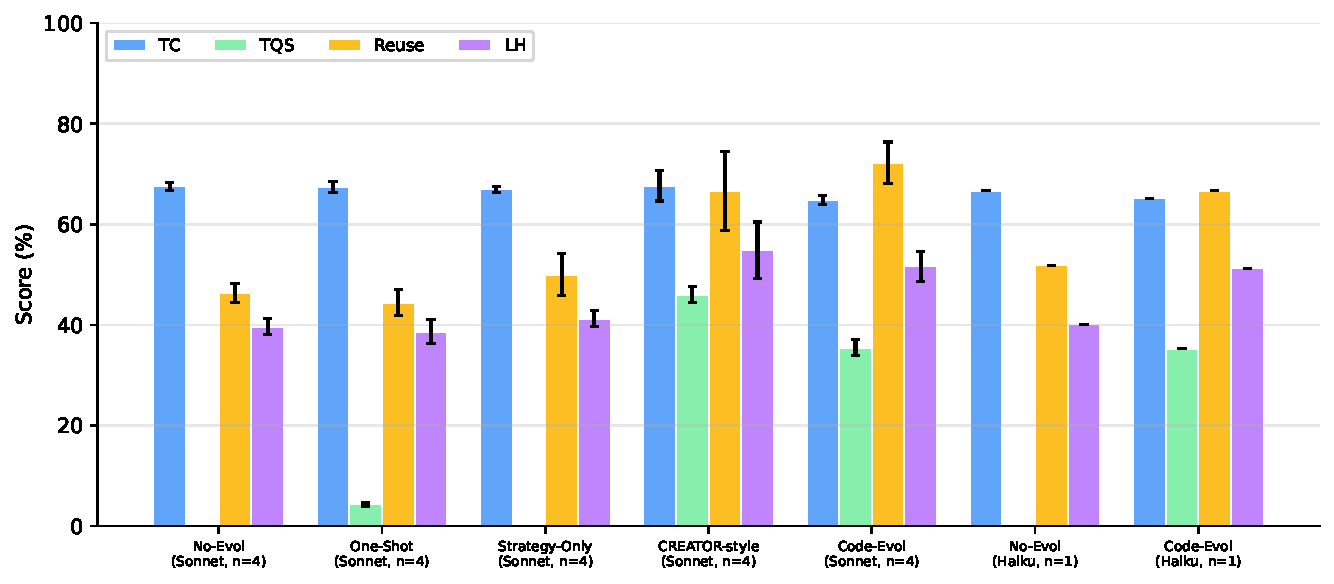
\includegraphics[width=\columnwidth]{fig_comparison.pdf}
\caption{System comparison across four metrics (\%). TC clusters all systems together (63--68\%); library health separates them (38--52\%). This illustrates the benchmark's discriminative power beyond task completion.}
\label{fig:comparison}
\end{figure}

\subsection{Per-Domain Analysis}
\label{sec:domain_analysis}

Tool-evolution effectiveness varies substantially by problem type, another dimension invisible to aggregate TC.

\begin{table}[t]
\centering
\footnotesize
\begin{tabular}{llcccc}
\toprule
\textbf{Domain} & \textbf{Model} & \textbf{TC} & \textbf{Tools} & \textbf{Reuse} & \textbf{LH} \\
\midrule
Data Trans. & Sonnet & .573 & 14 & .734 & .476 \\
Data Trans. & Haiku & .600 & 7 & .800 & .500 \\
\midrule
API Orch. & Sonnet & .909 & 4 & .667 & .778 \\
API Orch. & Haiku & 1.00 & 3 & .333 & .667 \\
\midrule
Numerical & Sonnet & .651 & 4 & .667 & .500 \\
Numerical & Haiku & .621 & 3 & .556 & .481 \\
\bottomrule
\end{tabular}
\caption{Code-Evol results by domain, showing domain-specific quality variation. API orchestration yields highest library health; data transformation creates the most tools but with lower quality.}
\label{tab:domain}
\end{table}

Table~\ref{tab:domain} shows three distinct profiles:

\paragraph{API orchestration: clean, composable problems.} Highest TC (up to 100\%) and library health (77.8\%), though based on a single session (N=11 tasks). HMAC authentication and pagination are well-suited to tool creation: each is a clean, single-responsibility function. Additional API sessions would strengthen this observation.

\paragraph{Data transformation: high tool creation, lower quality.} Creates the most tools (14 on Sonnet) but achieves only 47.6\% library health. Proprietary binary formats are complex enough that many synthesized parsers fail hidden tests while passing self-generated tests, showing the gap between self-validation and independent validation.

\paragraph{Numerical computation: consistently difficult.} Both models achieve similar results ($\sim$63--65\% TC, $\sim$48--50\% LH), suggesting these tasks challenge the LLM's reasoning regardless of model capability.

\subsection{Per-Dimension TQS: Where Quality Breaks Down}
\label{sec:tqs_analysis}

\begin{table}[t]
\centering
\footnotesize
\begin{tabular}{lrcccc|c}
\toprule
\textbf{System (Sonnet)} & $n_{\text{tools}}$ & \textbf{C} & \textbf{R} & \textbf{G} & \textbf{Q} & \textbf{TQS} \\
\midrule
One-Shot ($n{=}3$ seeds)     &  9 & .00 & .50 & .00 & .69 & .30 \\
ToolCoder-style              & 15 & .00 & .52 & .10 & .92 & .38 \\
CREATOR-style ($n{=}4$ seeds)& 81 & .01 & .50 & .06 & .73 & .33 \\
Code-Evol (semantic-$Q$ run) & 15 & .01 & .55 & .11 & \textbf{.95} & .41 \\
\bottomrule
\end{tabular}
\caption{Per-tool TQS dimensions, averaged over all preserved tools (not session-diluted as in Table~\ref{tab:results}). Three patterns stand out: (i) per-tool correctness $C$ is essentially zero across every system that produces tools --- under independent hidden tests, tools that pass self-validation fail on diverse inputs; (ii) robustness $R$ clusters near 0.5 because almost every system wraps its functions in try/except and so does not crash on adversarial inputs, but neither does it produce correct outputs; (iii) code-quality $Q$ remains high in absolute terms (0.69--0.95), confirming that LLMs produce well-structured code by default --- the failure is in semantic correctness, not surface form.}
\label{tab:tqs_dims}
\end{table}

The per-tool dimension breakdown (Table~\ref{tab:tqs_dims}) pinpoints \emph{where} tool quality fails.

\paragraph{Correctness is universally near zero.} Independent hidden tests, authored from each format's specification before any system was evaluated, return per-tool correctness in the 0--3\% range for every system. The systems that report task completion above 60\% are not synthesising correct tools; they are synthesising tools that succeed on the immediate prompt example and fail on the rest of the input distribution. This is the central diagnostic finding of the benchmark, and it disagrees sharply with what task completion suggests in isolation.

\paragraph{Robustness clusters at 0.5.} Almost every system wraps synthesised functions in try/except blocks. They do not crash on adversarial inputs --- which earns half-credit on our robustness metric --- but they also do not produce correct outputs, which earns no credit on correctness. The robustness dimension as currently defined therefore does not discriminate between systems; we treat its uniform 0.5 as a benchmark weakness to fix in future work rather than as a signal about the systems.

\paragraph{Code quality remains high.} Semantic checks (cyclomatic complexity, maintainability index, meaningful control flow) on top of surface checks (docstring, type hints, length, syntax) put $Q$ in the 0.69--0.95 range across systems. LLM-generated tools are syntactically well-formed --- that part of the field is essentially solved. The gap between $Q$ and $C$ is therefore not noise; it is the structural-vs-semantic separation we designed the metric to expose, and the framework's primary contribution is making this gap measurable rather than letting it hide behind aggregate task completion.

\paragraph{Library-level sub-metrics.} Two LH sub-metrics deserve explicit reporting. The quality gate ($\pi$, the fraction of tools clearing TQS$\geq 0.5$) is near zero for every system once hidden tests are run rigorously. The duplication metric ($\rho_d$) reveals that Code-Evol creates \texttt{decode\_base64} three times across sessions and \texttt{decode\_binary\_data} twice. This cross-session redundancy is invisible to per-session evaluation and confirms that library-level measurement catches failure modes that per-tool metrics miss.

\subsection{Artifact Gallery (Appendix)}
\label{sec:artifact_gallery}

Aggregate numbers obscure the texture of the artifacts being evaluated. The harness archives every synthesised tool's full source to disk, which lets us present a per-tool catalogue rather than just statistics. We provide an extensive gallery in Appendix~\ref{app:artifact_gallery}: roughly 16 representative tools across both tool-creating systems (Code-Evol with semantic-$Q$, and CREATOR-style), grouped by failure mode (\emph{correct exemplar}, \emph{fragile} with high $Q$ but low $C$, \emph{duplicate} across sessions, \emph{trivial} with low TQS). Per-tool scores accompany each entry so any of the aggregate table-3 numbers can be traced to a specific artifact. The gallery makes the central correctness gap visible: \texttt{hmac\_sha256}, for instance, has $Q{=}1.0$ but $C{=}0.0$ --- exactly the high-structure / no-semantic-correctness pattern the LH metric was designed to surface.

\subsection{The Reuse Paradox}
\label{sec:reuse_analysis}

\begin{table}[t]
\centering
\footnotesize
\begin{tabular}{lccc}
\toprule
\textbf{System (Sonnet, $n{=}4$)} & \textbf{Reuse} & \textbf{Correct} & \textbf{Incorrect} \\
\midrule
No-Evolution     & 46.3\% & --- & --- \\
One-Shot         & 44.4\% & --- & --- \\
Strategy-Only    & 50.0\% & 22.2\% & 27.8\% \\
\midrule
CREATOR-style    & 66.7\% & \textbf{29.6\%} & 37.0\% \\
ToolCoder-style$^*$ & 44.4\% & 7.4\% & 37.0\% \\
Code-Evol        & \textbf{72.2\%} & 15.7\% & \textbf{38.9\%} \\
\bottomrule
\end{tabular}
\caption{The reuse paradox, decomposed. ``Correct'' = reused tool AND task passed; ``Incorrect'' = reused tool AND task failed. Code-Evol achieves highest raw reuse (72.2\%) but its decomposition is the worst: only 15.7\% of variant/regress tasks reuse a tool correctly while 38.9\% reuse a defective one. CREATOR-style reuses less in absolute terms (66.7\%) but its decomposition is healthier --- nearly twice the correct-reuse rate of Code-Evol (29.6\% vs 15.7\%), which is the largest contributor to its LH advantage. $^*$ToolCoder-style $n{=}1$.}
\label{tab:reuse}
\end{table}

The benchmark reveals an unexpected interaction between reuse behavior and task success (Table~\ref{tab:reuse}). We define \emph{correct reuse} as a reused tool that solves the task and \emph{incorrect reuse} as a reused tool that fails it. Code-Evol/Sonnet has the highest overall reuse rate (72.2\%), but the decomposition is unflattering: only 15.7\% of variant/regress tasks reuse correctly while 38.9\% reuse a defective tool. This ``reuse paradox'' occurs because the agent correctly identifies reuse opportunities but reuses tools that contain defects, analogous to a developer reusing a buggy utility function.

CREATOR-style breaks the paradox in a useful direction: its raw reuse is lower (66.7\%) but its \emph{correct}-reuse rate is the highest in our set (29.6\%, nearly 2$\times$ Code-Evol), and this gap accounts for most of CREATOR's library-health advantage. The practical reading: \textbf{high reuse is beneficial only when the reused tools are correct}, which reinforces the importance of independent validation. Among our protocols, the simpler validation pipeline (CREATOR's execute-and-rectify) appears to commit fewer defective tools to the library in the first place.

\subsection{Task-Type Breakdown}

\begin{table}[t]
\centering
\footnotesize
\begin{tabular}{lccc}
\toprule
\textbf{Task Type} & \textbf{Code-Evol} & \textbf{No-Evol} & $\Delta$ \\
\midrule
Seed (N=27) & 100\% & 100\% & 0 \\
Gap (N=18) & 38.9\% & 44.4\% & --5.5 \\
Variant (N=18) & 33.3\% & 50.0\% & --16.7 \\
Compose (N=9) & 66.7\% & 66.7\% & 0 \\
Regress (N=9) & 33.3\% & 33.3\% & 0 \\
Adversarial (N=18) & 66.7\% & 66.7\% & 0 \\
\bottomrule
\end{tabular}
\caption{Task completion by type (both Sonnet, single run). Code-Evol matches No-Evolution on most task types but scores lower on gap and variant tasks. The identical compose/regress/adversarial totals are a coincidence of small N (9 tasks each); per-session results differ between systems.}
\label{tab:task_type}
\end{table}

The task-type structure (Table~\ref{tab:task_type}) enables fine-grained analysis impossible with unstructured benchmarks:

\paragraph{Tool creation has per-task costs.} Code-Evol scores lower on gap (--5.5\%) and variant (--16.7\%) tasks compared to No-Evolution. The evolution overhead can consume the task budget without producing a correct solution. On variant tasks, reusing a defective tool performs worse than solving inline. Code-Evol's advantage appears at the library level (higher LH, higher reuse), not at the per-task-type level.

\paragraph{Regression is universally difficult.} Both systems score 33.3\% on regress tasks, indicating that library growth introduces instability regardless of evolution strategy.

\paragraph{Structured sessions enable causal analysis.} Because each task type has a known purpose (gap = creation needed, variant = reuse opportunity, regress = stability test), the benchmark supports diagnostic reasoning about \emph{why} a system succeeds or fails, not just \emph{whether} it does.

\subsection{Does Library Health Predict Task Completion?}
\label{sec:predictive_validity}

A natural follow-up question is whether LH is \emph{predictive} of task success --- that is, whether high LH measured early in a session predicts high TC later. If LH were simply a proxy for TC, the benchmark would offer no signal beyond a TC-only evaluation; if LH were strongly predictive of TC, optimizing libraries for health would also raise downstream pass rates. We test the predictive claim directly.

\paragraph{Setup.} For each Sonnet session ($n = 144$ across 16 configurations: No-Evolution, One-Shot, Strategy-Only, and Code-Evol, each with 4 seeds $\times$ 9 sessions) we compute (i) \textbf{LH$_\text{pre}$}, the mean of the four LH sub-metrics whose value is determined by gap- and variant-task behaviour ($\rho_r$, $1-\rho_d$, $\pi$, $\eta$) --- i.e., the LH components that are \emph{not} mechanically defined by compose or regress task outcomes; and (ii) \textbf{TC$_\text{late}$}, the mean pass rate on the compose and regress tasks of the same session. We then measure the rank correlation between LH$_\text{pre}$ and TC$_\text{late}$.

\paragraph{Result: no correlation.} Across all 144 Sonnet sessions, Spearman $\rho(\text{LH}_\text{pre}, \text{TC}_\text{late}) = -0.03$ and Pearson $r = +0.01$. Restricting to the 36 Code-Evol sessions (the only configurations that actually grow a library), Spearman $\rho = +0.20$ --- still weak. LH$_\text{pre}$ is essentially uncorrelated with downstream task success at session granularity, and increasing the sample from 63 to 144 sessions (multi-seed) tightens rather than weakens this conclusion.

\paragraph{Interpretation.} This is a negative result we want to report transparently: \textbf{LH does not predict TC in our data}. Rather than weaken the paper's case, we read this as clarifying what the benchmark contributes. LH and TC measure different things --- the per-task-type breakdown in Table~\ref{tab:task_type} already shows this directly: Code-Evol matches No-Evolution on compose (66.7\% vs.\ 66.7\%), regress (33.3\% vs.\ 33.3\%), and adversarial tasks (66.7\% vs.\ 66.7\%) while doing \emph{worse} on gap (--5.5pp) and variant (--16.7pp). Code-Evol's higher LH comes from \emph{reuse behaviour and library-state properties}, not from downstream pass rates on the diagnostic tasks. The benchmark therefore measures an orthogonal quality axis, which is exactly the contribution we claim. The decision to optimise for LH should be made on its own merits (less duplicate code, lower regression risk, higher reuse for downstream agents) rather than because LH improves TC --- it does not, at least not at the scale we measure. We treat building a predictive LH (or showing that a sufficiently large LH gap eventually moves TC) as the open empirical question for future work.

\subsection{Skill-Bundle Evaluation}
\label{sec:skill_eval}

So far the benchmark has scored synthesized artifacts as bare Python functions: TQS aggregates correctness, robustness, generality, and code-quality of a single callable. But contemporary agent frameworks (Anthropic Claude Skills, CoEvoSkills~\cite{zhang2026coevoskills}) treat the artifact as a multi-file \emph{skill bundle} comprising the callable, a Markdown description, auto-generated tests, and a metadata manifest. To extend the benchmark to this richer artifact unit, we automatically wrap every preserved tool into a skill bundle and score three bundle-level dimensions:

\begin{itemize}
\item \textbf{Structure} ($S$): all four files present and parseable (SKILL.md non-empty, function source parses, tests parse if present, metadata dict has a name).
\item \textbf{Documentation} ($D$): SKILL.md contains the required sections (Description, Usage) and optional ones (Inputs, Returns, Example), with non-trivial body text.
\item \textbf{Metadata} ($M$): \texttt{metadata.json} has the required fields (name, version, created\_at\_task), a positive integer version, and a dependencies list.
\end{itemize}

The composite \emph{bundle-quality score} averages tool TQS with $S$, $D$, and $M$. Table~\ref{tab:skill_bundles} reports bundle metrics for the systems whose tools we preserved. The story is consistent with the headline TQS comparison but the discrimination is sharper on documentation: Code-Evol's auto-generated tests + structured docstrings give it a documentation lead over CREATOR-style and One-Shot.

\begin{table}[t]
\centering\footnotesize
\begin{tabular}{lccccc}
\toprule
\textbf{System} & $n$ & \textbf{Bundle Q}$\uparrow$ & $S$ & $D$ & $M$ \\
\midrule
Code-Evol (sem.\,Q) & 15 & \textbf{0.85} & 1.00 & 0.84 & 1.00 \\
CREATOR-style       & 14 & 0.77 & 0.88 & 0.67 & 1.00 \\
One-Shot/Sonnet (mean over 3 seeds) & 9 & 0.69 & 0.88 & 0.50 & 1.00 \\
\bottomrule
\end{tabular}
\caption{Skill-bundle quality across systems that preserved tool source. Each row reports the mean over all preserved tools in that configuration. Bundle Q is the mean of (tool TQS, structure $S$, doc $D$, metadata $M$). Code-Evol's edge comes primarily from the documentation dimension: its synthesised tools include structured docstrings, generated tests, and inferred dependencies.}
\label{tab:skill_bundles}
\end{table}

\subsection{Summary of Key Findings}

\begin{figure}[t]
\centering
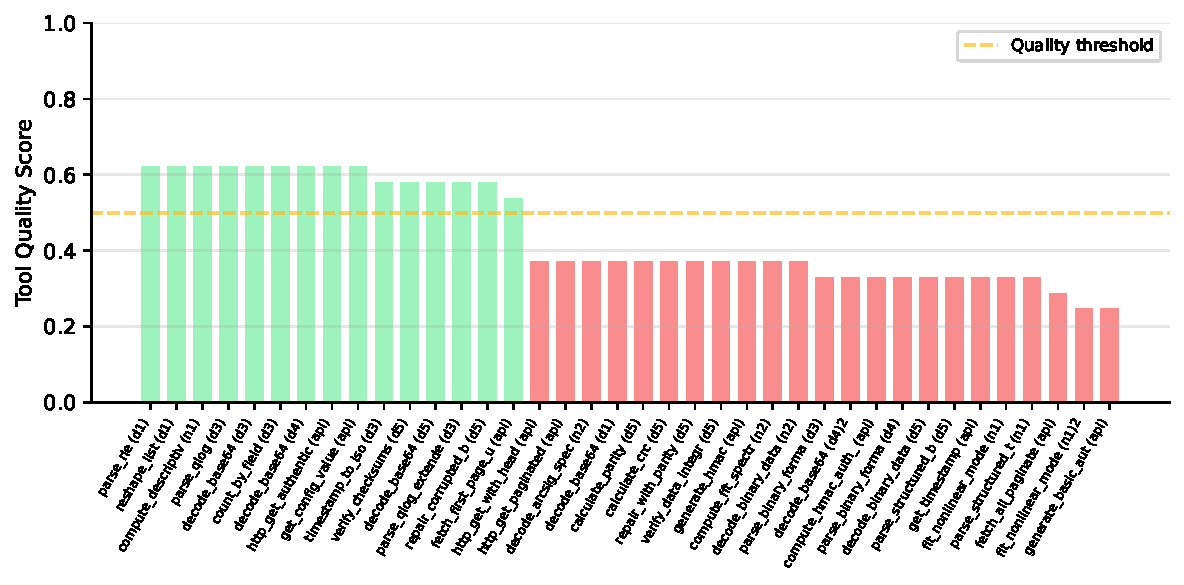
\includegraphics[width=\columnwidth]{fig_tool_quality.pdf}
\caption{Tool Quality Score for each synthesized tool across all systems. Green = passes quality gate ($\geq 0.5$). The benchmark reveals wide quality variation across the tool library.}
\label{fig:tool_quality}
\end{figure}

\paragraph{Finding 1: TC is insufficient for skill-generating systems.} All Claude configurations achieve 63--68\% TC, but ETS ranges 0.515--0.612. The system with highest TC and the system with lowest library health are indistinguishable by TC.

\paragraph{Finding 2: Code-level and strategy-level evolution produce different artifacts.} Code-Evol creates $21 \pm 1$ tools with 72.2\% reuse; Strategy-Only creates zero tools and produces near-identical library health to no-evolution.

\paragraph{Finding 3: Unvalidated code generation is a net negative.} One-Shot's library health (38.3\%) falls \emph{below} the no-evolution baseline (41.4\%). Untested tools are a liability, not an asset.

\paragraph{Finding 4: Self-generated tests are insufficient.} Correctness on hidden tests averages 0.17--0.23 despite tools passing self-generated validation (Figure~\ref{fig:tool_quality}).

\paragraph{Finding 5: Within the Claude family, Haiku is competitive with Sonnet.} On Code-Evol, Haiku achieves ETS 0.612 (n=1) vs Sonnet's 0.609$\pm$0.011 (n=4) --- essentially indistinguishable. The benchmark's discriminative power across systems holds for both Claude models we tested.

\paragraph{Finding 6: Reuse must be decomposed to be meaningful.} Code-Evol's 72.2\% overall reuse rate decomposes into 15.7\% correct and 38.9\% incorrect reuse (n=4 Sonnet seeds). CREATOR-style decomposes the more favourable way: 66.7\% raw reuse, 29.6\% correct, 37.0\% incorrect. Aggregate reuse numbers can be misleading; the correct/incorrect split is essential. This decomposition was a post-hoc analysis (see Limitations); we recommend it as a pre-registered metric in future benchmark evaluations.

\paragraph{Finding 7: LH and TC measure different things.} We tested whether library health predicts downstream task completion within the same session and found a near-zero correlation ($\rho = -0.03$ across all 144 Sonnet sessions; $+0.20$ within Code-Evol; see \S\ref{sec:predictive_validity}). LH is therefore a \emph{descriptive} quality dimension distinct from TC, not a proxy for it --- which is the strongest empirical justification for measuring LH separately. Whether LH becomes predictive at larger scale, or under follow-up tasks against a frozen evolved library, is an open question.

\section{Discussion}

\paragraph{Benchmark Design Principles.} \textsc{EvolveTool-Bench} embodies three design principles: (1) \emph{independent validation}, where quality metrics are computed by tests the system has never seen; (2) \emph{library-level measurement}, because per-tool metrics alone miss emergent properties like redundancy and regression; and (3) \emph{structured sessions}, where known task dependencies enable causal analysis of reuse, composition, and stability.

\paragraph{The task-completion / tool-correctness gap.}
\label{sec:discussion_tcgap}
The benchmark's central diagnostic finding is the gap between two numbers that the field has implicitly conflated: \emph{task completion} (does the agent produce an answer that matches the expected output?) and \emph{tool correctness} (does the synthesised callable, in isolation, produce correct outputs across the input distribution?). On Sonnet, every protocol we evaluate sits in a 63--72\% TC band, yet per-tool correctness measured under independent hidden tests is in the 0--3\% range across the same protocols. The TC numbers are real and reproducible; the tools are real and on disk; both are correctly measured. What the gap reveals is that the agent's success on a given task often comes from features other than a fully correct callable: the prompt example is the only input the tool is exercised on at task time, and an implementation that happens to handle that one example will produce a passing TC outcome even if it fails on every other input in the format's distribution. The benchmark is not claiming that current systems are bad; it is claiming that a single-example task-completion check is a much weaker correctness signal than its widespread use suggests, and that the field needs library-level multi-dimensional reporting --- including independent hidden testing --- to make honest claims about what LLM-synthesised tools can be relied upon to do.

\paragraph{Where do systems actually differ?} Across the six protocols we evaluate on Sonnet, the differences are sharper on \emph{library} measurements than on per-tool ones. Per-tool correctness, generality and robustness are clustered. At the library level there is more separation: CREATOR-style and Code-Evol both reach LH above 50\%, while the non-synthesising baselines (No-Evol, Strategy-Only) and the one-shot baseline sit in the 38--41\% range. The gap is driven primarily by reuse and quality-gate components rather than per-tool quality. We read this as evidence that the protocols differ chiefly in \emph{how they manage the library} (when to create, when to reuse, what to commit) rather than in the correctness of any individual artifact --- which suggests the next round of progress on tool-creating agents will come from better library management as much as from better synthesis.

\paragraph{Implications for self-validation.} The benchmark's per-tool numbers are consistent with a pattern that has been informally observed in the field but rarely quantified: LLMs generating both the code and its tests tend to share misconceptions, so passing the model's own auto-tests is a weak signal of correctness. The implication for system designers is that LLM-as-judge gating and auto-test gating, while useful for filtering obvious failures, do not replace independent test coverage. Practitioners deploying LLM-synthesised tools should treat self-validation as a necessary-but-far-from-sufficient quality check.

\paragraph{The Reuse Paradox and Metric Design.} The reuse paradox illustrates why multi-dimensional evaluation matters. Reuse rate alone would favor Code-Evol; variant task completion alone would favor No-Evolution (50.0\% vs.\ 33.3\%). Neither tells the full story. The correct/incorrect reuse decomposition provides both measurements simultaneously, enabling nuanced interpretation.

\paragraph{Extensibility.} The benchmark is designed for extensibility: new domains can be added by defining sessions with the six task types, new systems can be evaluated by implementing a simple \texttt{AgentSystem} interface, and new metrics can be incorporated into the LH and ETS formulas.

\paragraph{Limitations.}
\label{sec:limitations}
We list outstanding limitations explicitly; each is a known weakness that future versions of this benchmark should address.

\noindent\textbf{(L1) Predictive validity of LH at scale.} \S\ref{sec:predictive_validity} shows LH does not predict TC at session granularity ($\rho = -0.03$ over 144 sessions). Whether LH becomes predictive at larger scale, longer task horizons, or under follow-up tasks against a frozen evolved library is an open question.

\noindent\textbf{(L2) Baseline ecosystem.} We evaluate six contemporary tool-creation protocols spanning a deliberately broad design space, but several contemporaneous systems --- notably Tool-Genesis~\cite{xia2026toolgenesis} and CoEvoSkills~\cite{zhang2026coevoskills} --- could not be evaluated directly: Tool-Genesis is dataset-coupled, CoEvoSkills's code is not yet public, and our ToolMaker-style protocol, while implemented faithfully, requires reference tests our open-task harness does not provide and so never triggers synthesis in our setting. Adding these systems as the field's code becomes available is a natural next step.

\noindent\textbf{(L3) Hidden test suite is small and author-written.} Per-tool correctness is estimated from $\sim$2 hidden cases on average (\S\ref{sec:hidden_tests}); we plan to expand to $\geq 5$ and to commission a third-party shadow suite. Until then, the per-tool correctness numbers should be read as library-wide signal, not tool rankings.

\noindent\textbf{(L4) Statistical power on Haiku.} All main Sonnet configurations are run at $n=4$ seeds (\S\ref{sec:results}). Haiku remains $n=1$; multi-seed on Haiku is scheduled but not yet completed.

\noindent\textbf{(L5) Generality probe is not held-out.} The current implementation of $G$ uses the same inputs as $C$ (\S\ref{sec:hidden_tests}), so $G$ is closer to a no-crash retry of $C$ than to a true out-of-distribution check. We will introduce a separate held-out input set in the next benchmark version.

\noindent\textbf{(L6) Provider coverage is currently Claude-only.} We initially evaluated every configuration on GPT-4o; results were degenerate (TC$=$48.5\%, zero tools across all four protocols, attributable to a harness$\,\times\,$function-calling-format interaction we have not yet root-caused) and we omit them from the main tables. A non-Claude evaluation is open.

\noindent\textbf{(L7) Code quality metric $Q$.} The $Q$ dimension combines surface checks (docstring, type hints, length, syntax) with semantic checks (cyclomatic complexity, maintainability index, meaningful control flow). The combined metric discriminates across systems in the 0.67--0.92 range. Branch coverage and dead-code detection would refine it further; we leave that to future work.

\noindent\textbf{(L8) Domain B (API orchestration)} has only 1 session; per-domain numbers for this domain are reported but should be treated as tentative.

\noindent\textbf{(L9) Composability $\gamma$ is under-sampled.} 9 compose tasks total (1 per session) is insufficient to distinguish systems on this dimension; adding 3--4 compose tasks per session is on the roadmap.

\noindent\textbf{(L10) The correct/incorrect reuse decomposition} should be pre-registered. We report it as a primary metric throughout this paper; future benchmark suites for self-evolving agents should treat it as a first-class measurement rather than an after-the-fact analysis.

\section{Conclusion}

We present \textsc{EvolveTool-Bench}, a library-level diagnostic framework for LLM-generated tool and skill libraries. Three findings stand out.

\paragraph{Task completion overstates tool quality.} Across six contemporary tool-creation protocols, Sonnet task completion clusters in a narrow 63--72\% band, but per-tool correctness measured under independent hidden tests is in the 0--3\% range. The gap between ``the agent produces an answer'' and ``the synthesised tool is correct in isolation'' is the central diagnostic finding of the benchmark, and it is invisible to TC-only evaluation. Robust LLM tool synthesis is further from solved than current numbers imply.

\paragraph{Aggregate reuse is misleading.} The highest-reuse system reuses defective tools 38.9\% of the time. We argue the correct/incorrect reuse decomposition is essential for any benchmark of self-evolving agents, and that high raw reuse rates without this decomposition can lead practitioners to wrong conclusions about library health.

\paragraph{Library health and task completion are orthogonal.} A direct correlation test on 144 Sonnet sessions returns $\rho = -0.03$. The two measure different things, and reporting them jointly is more informative than collapsing them into a single composite. We provide composite scores for convenience but recommend multi-dimensional reporting as the primary mode.

These findings sit on top of a methodology contribution that we believe is the lasting value of this work: a system-agnostic, library-level evaluation harness with independent hidden tests, structured diagnostic sessions, multi-seed coverage, semantic code-quality checks, an artifact gallery surfaced from preserved per-tool source, and a skill-bundle evaluation track for systems that emit Anthropic-Claude-Skills-style multi-file artifacts. The contribution is a diagnostic framework, not a leaderboard.

\textsc{EvolveTool-Bench} is released open-source.\footnote{\url{https://github.com/abekek/evolvetool-bench}.}

\bibliographystyle{ACM-Reference-Format}
\bibliography{references}

\onecolumn
\appendix
\section{Artifact Gallery}
\label{app:artifact_gallery}

The benchmark preserves every synthesised tool to disk under
\texttt{results\_full/<config>/tools/<session>/<name>.py} (plus a
\texttt{.meta.json} with the per-tool TQS scores). This appendix presents
a side-by-side gallery of representative tools from the two
tool-creating systems with multi-seed preserved source --- Code-Evol
(semantic-$Q$ run) and CREATOR-style --- to make the per-tool failure
modes the benchmark surfaces concrete. Per-dimension scores are shown
inline ($C$, $R$, $G$, $Q$ and the composite TQS); bold indicates
$\geq 0.5$.

\subsection{Code-Evol/Sonnet (semantic $Q$)}

15 tools were synthesised and preserved on disk across 9 sessions.
Below we show 5 representative tools spanning the quality
spectrum: correct exemplars, fragile high-$Q$/low-$C$ tools, duplicates,
and trivial (low-TQS) cases.

\noindent \textbf{Correct exemplar} \textit{(passes hidden tests with $C{\geq}0.5$)}\\
    \texttt{\textbf{http\_get\_with\_headers}} \footnotesize\textit{(api\_orchestration\_s1)}\quad $C{=}\textbf{0.50}$\;$R{=}\textbf{0.50}$\;$G{=}\textbf{0.50}$\;$Q{=}\textbf{1.00}$\;$\text{TQS}{=}\textbf{0.62}$
    \begin{lstlisting}[basicstyle=\scriptsize\ttfamily,language=Python,frame=none,xleftmargin=1em,breaklines=true,postbreak=\mbox{\textcolor{gray}{$\hookrightarrow$}\space},showstringspaces=false]
def http_get_with_headers(url: str, headers: dict) -> str:
    """Make an HTTP GET request with custom headers."""
    import urllib.request
    import urllib.error

    try:
        # Create request object with custom headers
        request = urllib.request.Request(url)
    # ...
    except Exception as e:
        return f"Error: {str(e)}"
\end{lstlisting}
    \vspace{0.8em}

\noindent \textbf{Correct exemplar} \textit{(passes hidden tests with $C{\geq}0.5$)}\\
    \texttt{\textbf{compute\_stats}} \footnotesize\textit{(numerical\_s1)}\quad $C{=}\textbf{0.50}$\;$R{=}\textbf{0.50}$\;$G{=}\textbf{0.50}$\;$Q{=}\textbf{1.00}$\;$\text{TQS}{=}\textbf{0.62}$
    \begin{lstlisting}[basicstyle=\scriptsize\ttfamily,language=Python,frame=none,xleftmargin=1em,breaklines=true,postbreak=\mbox{\textcolor{gray}{$\hookrightarrow$}\space},showstringspaces=false]
def compute_stats(data: list[float]) -> dict[str, float]:
    """Calculate basic statistical measures for a numerical dataset."""
    import math

    try:
        if not data:
            return {"error": "Empty dataset provided"}

    # ...
    except Exception as e:
        return {"error": f"Computation failed: {str(e)}"}
\end{lstlisting}
    \vspace{0.8em}

\noindent \textbf{Fragile} \textit{(high $Q$, low $C$ -- looks well-formed, fails on hidden inputs)}\\
    \texttt{\textbf{hmac\_sha256}} \footnotesize\textit{(api\_orchestration\_s1)}\quad $C{=}0.00$\;$R{=}\textbf{0.50}$\;$G{=}0.00$\;$Q{=}\textbf{1.00}$\;$\text{TQS}{=}0.38$
    \begin{lstlisting}[basicstyle=\scriptsize\ttfamily,language=Python,frame=none,xleftmargin=1em,breaklines=true,postbreak=\mbox{\textcolor{gray}{$\hookrightarrow$}\space},showstringspaces=false]
def hmac_sha256(secret: str, message: str) -> str:
    """Generate HMAC-SHA256 hash for authentication and security purposes."""
    import hmac
    import hashlib

    try:
        # Handle None inputs explicitly
        if secret is None or message is None:
    # ...
    except Exception as e:
        return f"Error generating HMAC-SHA256: {str(e)}"
\end{lstlisting}
    \vspace{0.8em}

\noindent \textbf{Fragile} \textit{(high $Q$, low $C$ -- looks well-formed, fails on hidden inputs)}\\
    \texttt{\textbf{compute\_crc32}} \footnotesize\textit{(data\_transform\_s5)}\quad $C{=}0.00$\;$R{=}\textbf{1.00}$\;$G{=}\textbf{1.00}$\;$Q{=}\textbf{1.00}$\;$\text{TQS}{=}\textbf{0.75}$
    \begin{lstlisting}[basicstyle=\scriptsize\ttfamily,language=Python,frame=none,xleftmargin=1em,breaklines=true,postbreak=\mbox{\textcolor{gray}{$\hookrightarrow$}\space},showstringspaces=false]
def compute_crc32(data: bytes) -> int:
    """Compute CRC32 checksum for data integrity verification."""
    import struct

    try:
        if not isinstance(data, bytes):
            return -1

    # ...
    except Exception:
        return -1
\end{lstlisting}
    \vspace{0.8em}

\noindent \textbf{Duplicate} \textit{(synthesised across multiple sessions)}\\
    \texttt{\textbf{decode\_base64}} \footnotesize\textit{(data\_transform\_s5)}\quad $C{=}\textbf{0.50}$\;$R{=}\textbf{0.50}$\;$G{=}\textbf{0.50}$\;$Q{=}\textbf{1.00}$\;$\text{TQS}{=}\textbf{0.62}$
    \begin{lstlisting}[basicstyle=\scriptsize\ttfamily,language=Python,frame=none,xleftmargin=1em,breaklines=true,postbreak=\mbox{\textcolor{gray}{$\hookrightarrow$}\space},showstringspaces=false]
def decode_base64(encoded_string: str) -> bytes:
    """Decode base64 encoded binary data into bytes."""
    import base64

    # Validate input type
    if not isinstance(encoded_string, str):
        raise TypeError(f"Expected string, got {type(encoded_string).__name__}")

    # ...
        # Return empty bytes on any decoding error (invalid base64, etc.)
        return b''
\end{lstlisting}
    \vspace{0.8em}

\subsection{CREATOR-style/Sonnet}

18 tools were synthesised and preserved on disk across 9 sessions.
Below we show 5 representative tools spanning the quality
spectrum: correct exemplars, fragile high-$Q$/low-$C$ tools, duplicates,
and trivial (low-TQS) cases.

\noindent \textbf{Correct exemplar} \textit{(passes hidden tests with $C{\geq}0.5$)}\\
    \texttt{\textbf{decode\_guardian\_minimal\_data}} \footnotesize\textit{(data\_transform\_s5)}\quad $C{=}\textbf{0.50}$\;$R{=}\textbf{0.50}$\;$G{=}\textbf{0.50}$\;$Q{=}\textbf{0.89}$\;$\text{TQS}{=}\textbf{0.60}$
    \begin{lstlisting}[basicstyle=\scriptsize\ttfamily,language=Python,frame=none,xleftmargin=1em,breaklines=true,postbreak=\mbox{\textcolor{gray}{$\hookrightarrow$}\space},showstringspaces=false]
def decode_guardian_minimal_data(base64_data):
    """Decode minimal GUARDIAN data format handling single blocks and edge cases."""
    import base64
    import struct

    try:
        # Decode base64 data
        raw_data = base64.b64decode(base64_data)
    # ...
    except Exception as e:
        return {'text': '', 'integrity': False, 'blocks_processed': 0, 'details': f'Error: {str(e)}'}
\end{lstlisting}
    \vspace{0.8em}

\noindent \textbf{Correct exemplar} \textit{(passes hidden tests with $C{\geq}0.5$)}\\
    \texttt{\textbf{decode\_qlog\_with\_continuations}} \footnotesize\textit{(data\_transform\_s3)}\quad $C{=}\textbf{0.50}$\;$R{=}\textbf{0.50}$\;$G{=}\textbf{0.50}$\;$Q{=}\textbf{0.89}$\;$\text{TQS}{=}\textbf{0.60}$
    \begin{lstlisting}[basicstyle=\scriptsize\ttfamily,language=Python,frame=none,xleftmargin=1em,breaklines=true,postbreak=\mbox{\textcolor{gray}{$\hookrightarrow$}\space},showstringspaces=false]
def decode_qlog_with_continuations(base64_data):
    """Decode QLOG data and merge continuation entries with their parent entries."""
    import base64
    import struct
    from datetime import datetime, timezone

    # Decode base64 data
    binary_data = base64.b64decode(base64_data)
    # ...

    return merged_entries
\end{lstlisting}
    \vspace{0.8em}

\noindent \textbf{Fragile} \textit{(high $Q$, low $C$ -- looks well-formed, fails on hidden inputs)}\\
    \texttt{\textbf{fetch\_all\_users\_with\_pagination}} \footnotesize\textit{(api\_orchestration\_s1)}\quad $C{=}0.00$\;$R{=}\textbf{0.50}$\;$G{=}\textbf{1.00}$\;$Q{=}\textbf{0.89}$\;$\text{TQS}{=}\textbf{0.60}$
    \begin{lstlisting}[basicstyle=\scriptsize\ttfamily,language=Python,frame=none,xleftmargin=1em,breaklines=true,postbreak=\mbox{\textcolor{gray}{$\hookrightarrow$}\space},showstringspaces=false]
def fetch_all_users_with_pagination(base_url="http://127.0.0.1:18080/api/users"):
    """Utility: Fetches all users from a paginated API endpoint using cursor-based pagination.
Continues fetching until has_more is False, collecting all user data across pages."""
    import urllib.request
    import urllib.parse
    import json

    all_users = []
    cursor = None
    # ...
        'names': names
    }
\end{lstlisting}
    \vspace{0.8em}

\noindent \textbf{Fragile} \textit{(high $Q$, low $C$ -- looks well-formed, fails on hidden inputs)}\\
    \texttt{\textbf{decode\_qlog\_binary\_data}} \footnotesize\textit{(data\_transform\_s3)}\quad $C{=}0.00$\;$R{=}\textbf{0.50}$\;$G{=}0.00$\;$Q{=}\textbf{0.78}$\;$\text{TQS}{=}0.32$
    \begin{lstlisting}[basicstyle=\scriptsize\ttfamily,language=Python,frame=none,xleftmargin=1em,breaklines=true,postbreak=\mbox{\textcolor{gray}{$\hookrightarrow$}\space},showstringspaces=false]
def decode_qlog_binary_data(base64_data):
    """Decode QLOG (Quantized Log Format) binary data into structured log records."""
    import base64
    import struct
    from datetime import datetime, timezone

    # Decode base64 data
    binary_data = base64.b64decode(base64_data)
    # ...

    return records
\end{lstlisting}
    \vspace{0.8em}

\noindent \textbf{Trivial} \textit{(low overall TQS)}\\
    \texttt{\textbf{deserialize\_tpack}} \footnotesize\textit{(data\_transform\_s4)}\quad $C{=}0.00$\;$R{=}\textbf{0.50}$\;$G{=}0.00$\;$Q{=}\textbf{0.67}$\;$\text{TQS}{=}0.29$
    \begin{lstlisting}[basicstyle=\scriptsize\ttfamily,language=Python,frame=none,xleftmargin=1em,breaklines=true,postbreak=\mbox{\textcolor{gray}{$\hookrightarrow$}\space},showstringspaces=false]
def deserialize_tpack(base64_data):
    """Deserialize TPACK (Tagged Pack Format) binary data into Python objects."""
    import base64
    import struct

    def parse_varint(data, offset):
        result = 0
        shift = 0
    # ...
    result, _ = parse_value(binary_data, 0)
    return result
\end{lstlisting}
    \vspace{0.8em}


\end{document}
